\section{Results}
\label{sec:result}
In this section we run six different case for DBSCAN algorithm some changes in input data and other in algorithm it self.all codes and implementation are done with python 3.8.5 and sklearn package\cite{scikit-learn}. you can see the experiments and their details in table \ref{tab:experiments}.
\begin{table}
	\centering
	\caption{Summery of designed experiments}
	\label{tab:experiments}
	\begin{tabular}{ll}\toprule
		\textbf{Experiment NO} & \textbf{Details}\\
		\midrule
		base & Bolbs dataset, $\epsilon$ = 3, MinPoint = 3\\ \midrule\midrule
		1 & No Structure \\
		2 & Noisy Moon dataset \\
		3 & Noisy Circles dataset \\ \midrule 
		4 &  Manhattan distance \\ 
		5 &  $ \epsilon = 0.5 $ \\
		6 &  MinPoint = 5 \\ \bottomrule
	\end{tabular}
\end{table}
We can see the result of clustering for base condition in figure \ref{fig:bolb} and its confusion matrix in figure \ref{fig:cmbolb}. the first row of confusion matrix is for noise data.
and then we run the algorithm in cases that we just change the input data but with the same algorithm parameter in base condition. the result is show in figure \ref{fig:panel1}.
\begin{figure}[h]
	\centering
	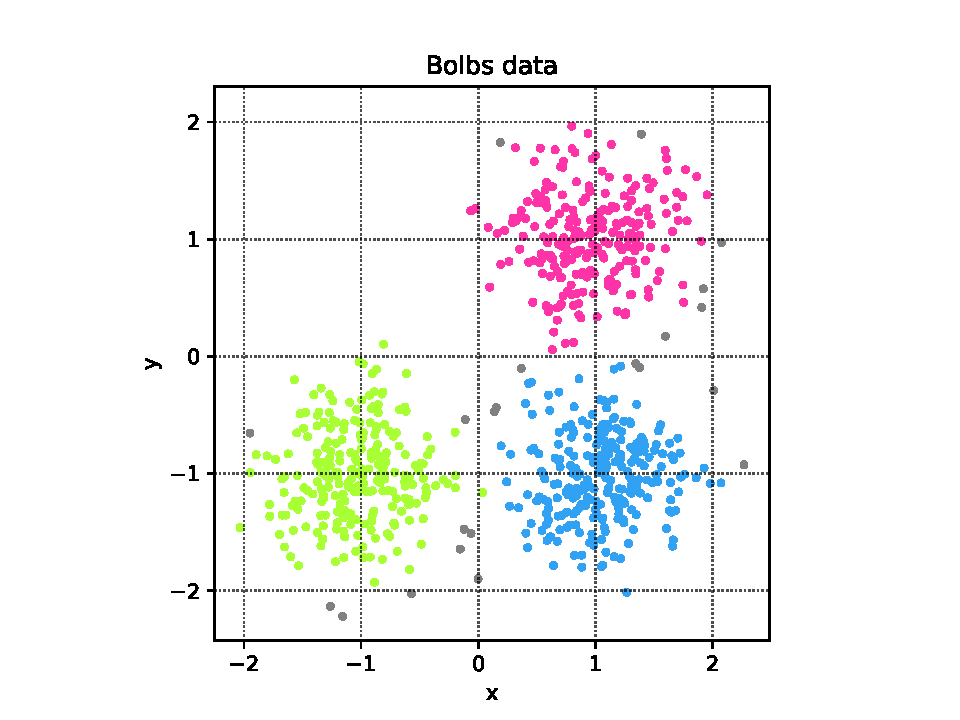
\includegraphics[width=1\linewidth]{figures/bolb}
	\caption{DBSCAN in base experiment, gray points are considered as noise}
	\label{fig:bolb}
\end{figure}
\begin{figure}[h]
	\centering
	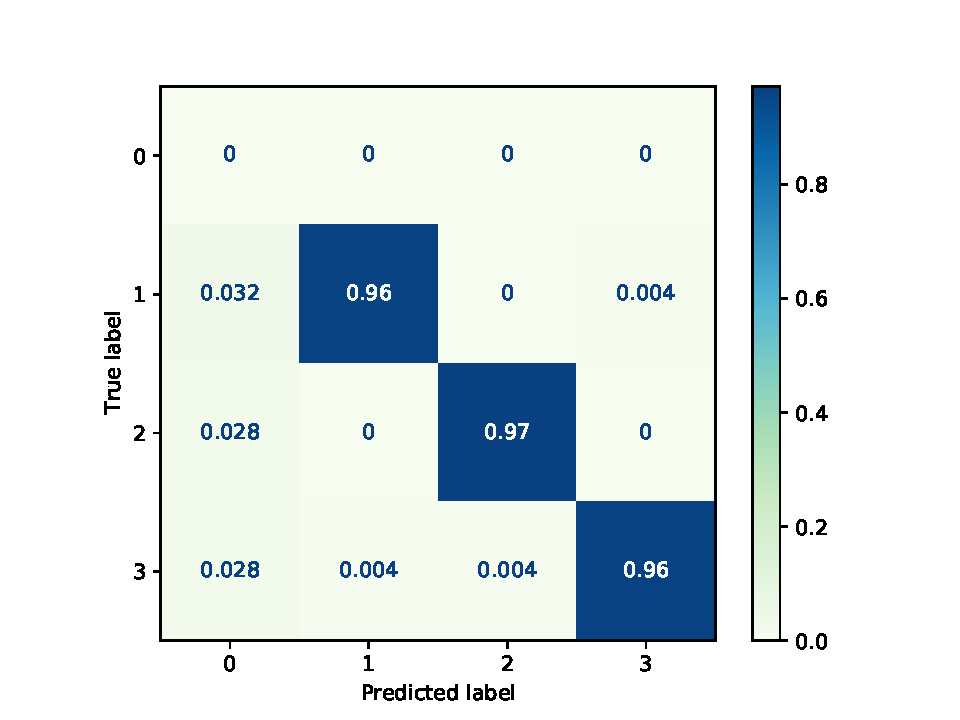
\includegraphics[width=1\linewidth]{figures/cm_bolb}
	\caption{Normalized confusion matrix}
	\label{fig:cmbolb}
\end{figure}

\begin{figure*}[h]
	\begin{subfigure}{0.33\linewidth}
		\centering
		% include first image
		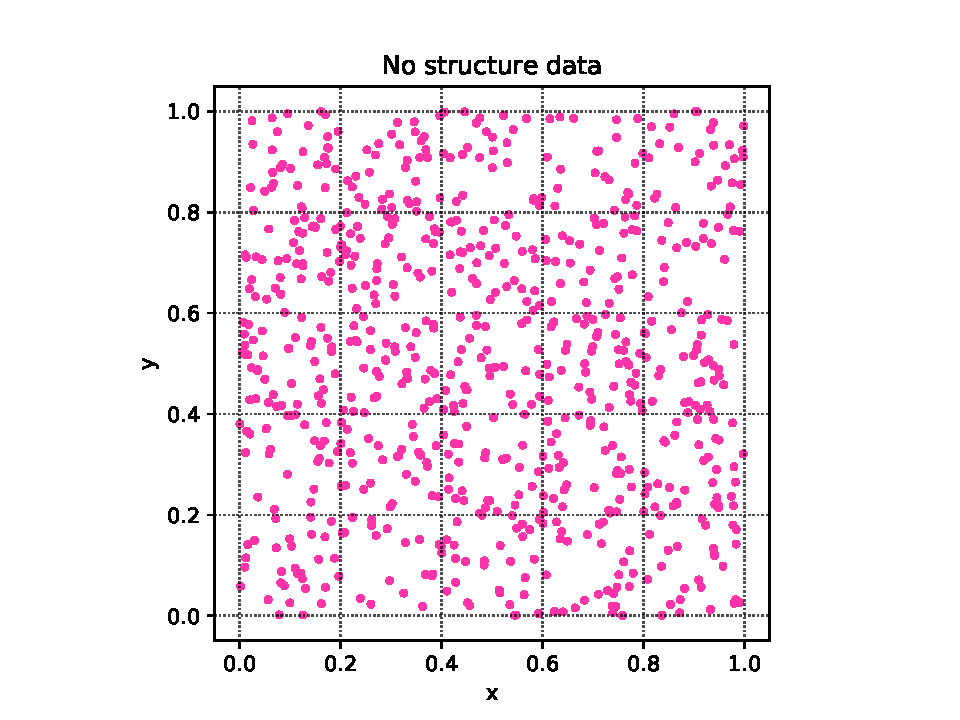
\includegraphics[width=\linewidth]{figures/1-NoStructure}  
		\caption{DBSCAN in first experiment}
		\label{fig:p1-1}
	\end{subfigure}
	\begin{subfigure}{0.33\textwidth}
		\centering
		% include image 2
		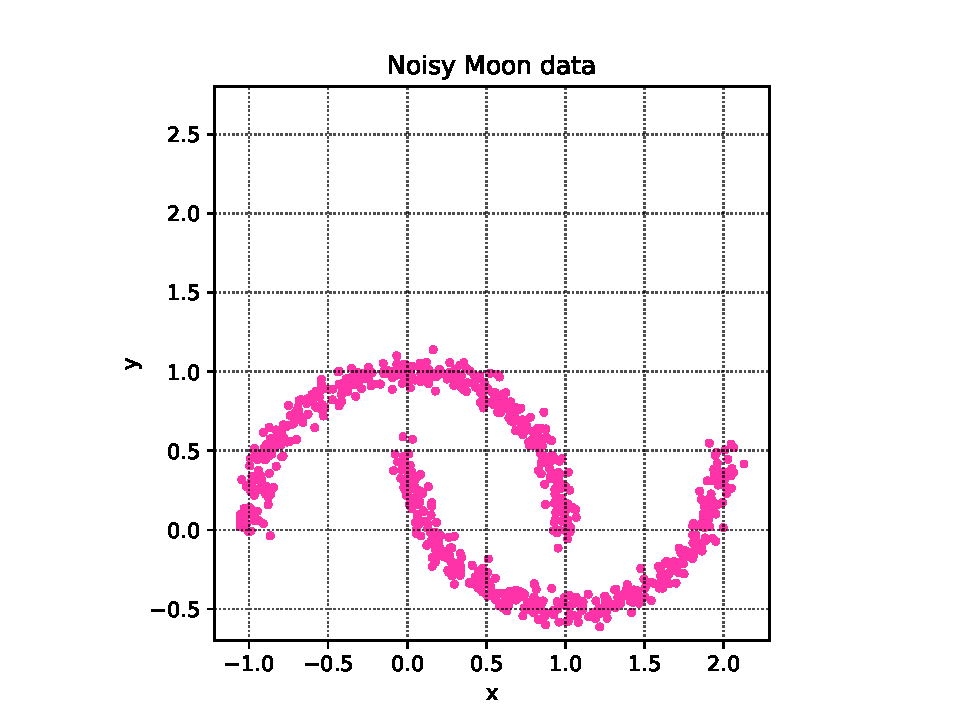
\includegraphics[width=\linewidth]{figures/2-NoisyMoon}
		\caption{DBSCAN in second experiment}
		\label{fig:p1-2}
	\end{subfigure}
	\begin{subfigure}{0.33\textwidth}
		\centering
		% include image 3
		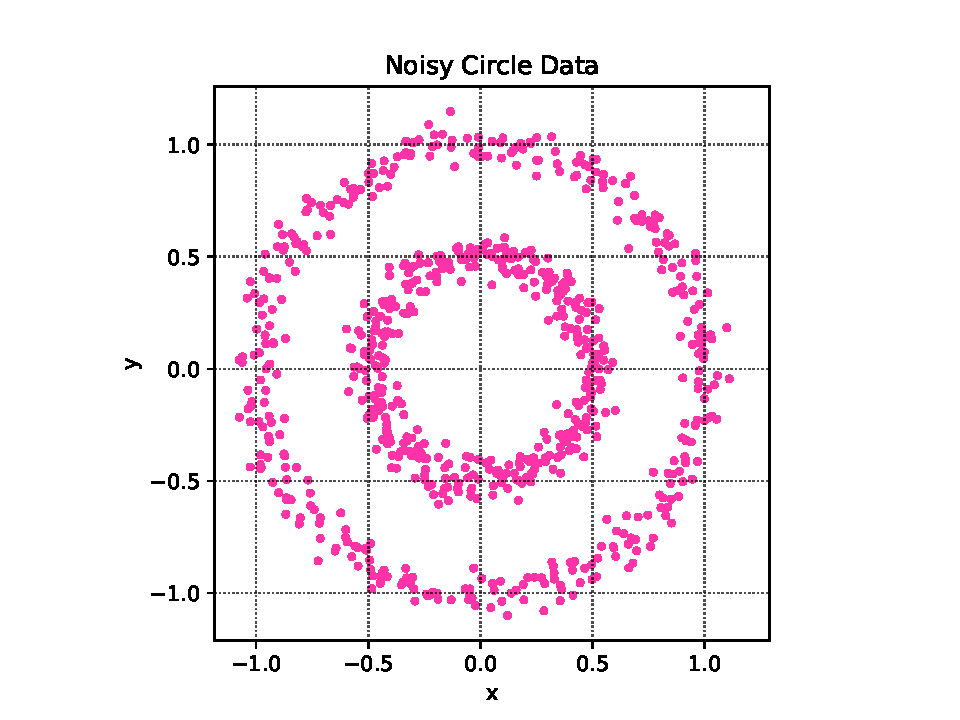
\includegraphics[width=\linewidth]{figures/3-NoisyCircle}
		\caption{DBSCAN in third experiment}
		\label{fig:p1-3}
	\end{subfigure}	
	
	
	\begin{subfigure}{0.33\textwidth}
		\centering
		% include image 4
		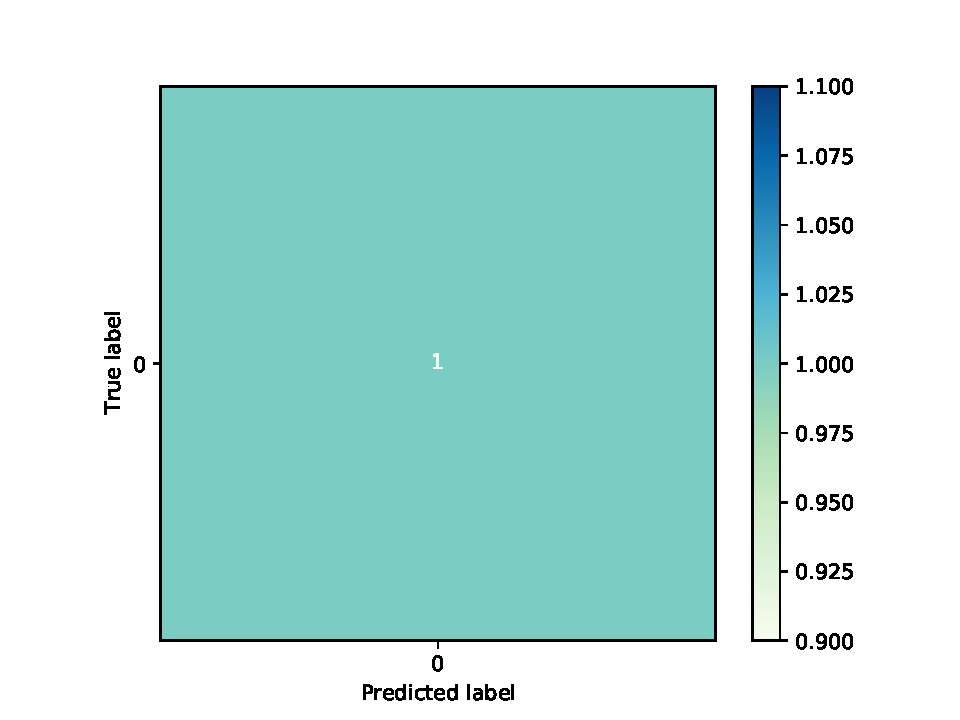
\includegraphics[width=\linewidth]{figures/1-cm-NoStructure}
		\caption{Confusion matrix of no structure data}
		\label{fig:p1-4}
	\end{subfigure}
	\begin{subfigure}{0.33\textwidth}
		\centering
		% include image 5
		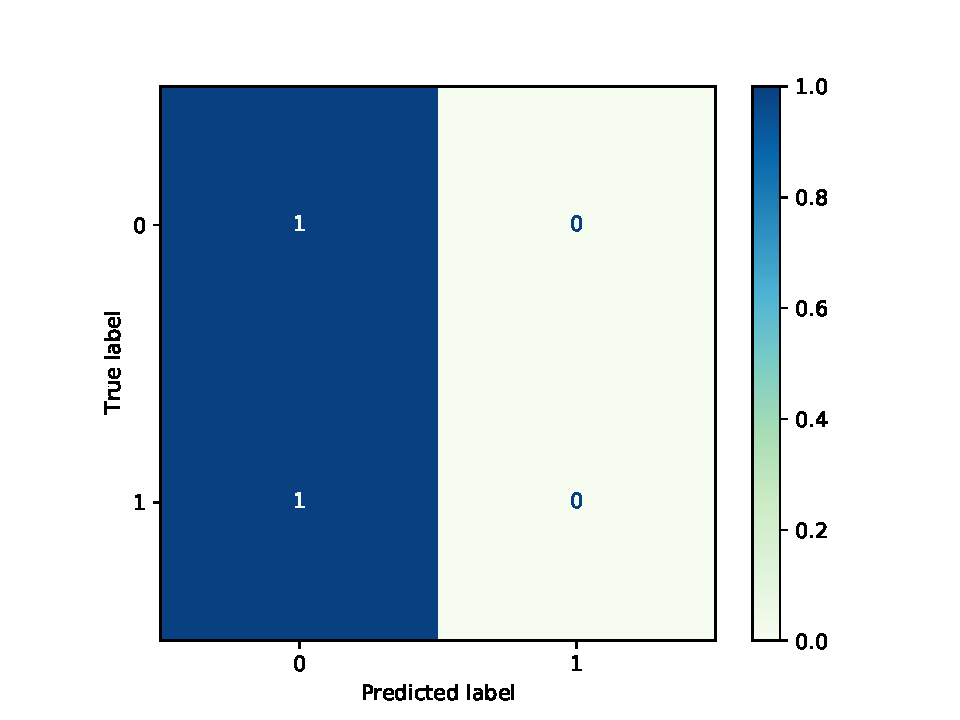
\includegraphics[width=\linewidth]{figures/2-cm-NoisyMoon}  
		\caption{Confusion matrix of noisy moon data}
		\label{fig:p1-5}
	\end{subfigure}
	\begin{subfigure}{0.33\textwidth}
		\centering
		% include image 6
		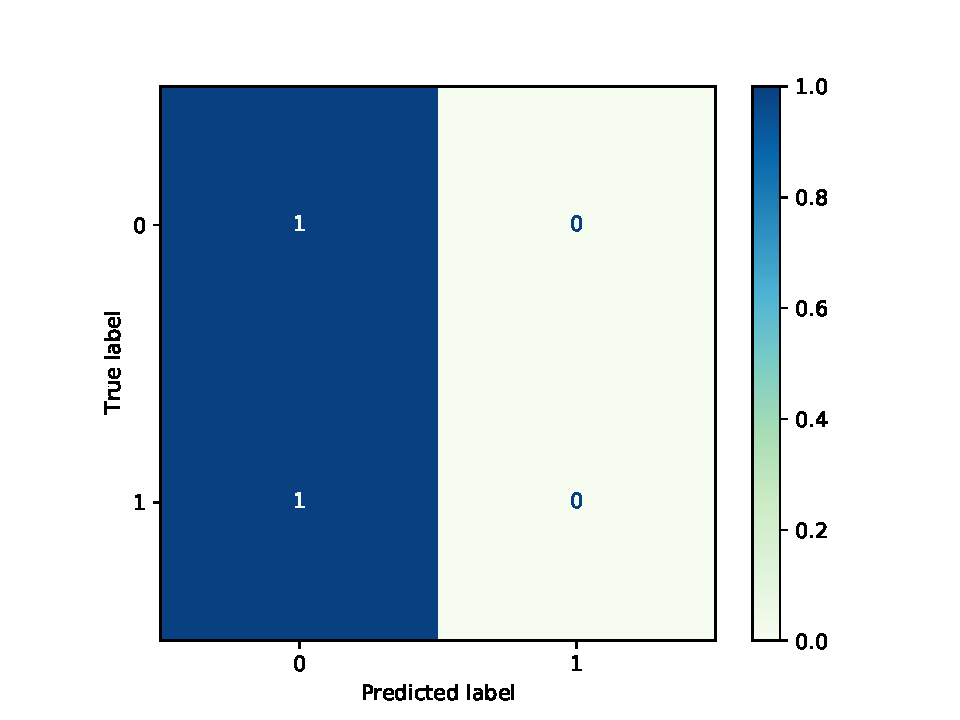
\includegraphics[width=\linewidth]{figures/3-cm-NoisyCircle}  
		\caption{Confusion matrix of noisy circle data}
		\label{fig:p1-6}
	\end{subfigure}
	\caption{Result of first \subref{fig:p1-1} three experiment as you can see in \cref{fig:p1-1,fig:p1-2} DBSCAN just found one cluster while there is two, and this is because of setting its parameters not precise.}
	\label{fig:panel1}
\end{figure*}
In figure \ref{fig:panel2} you can see the results when we change the parameters of algorithm such as metric function, $\epsilon$ and MinPoint.
\begin{figure*}[h]
	\begin{subfigure}{0.33\textwidth}
		\centering
		% include first image
		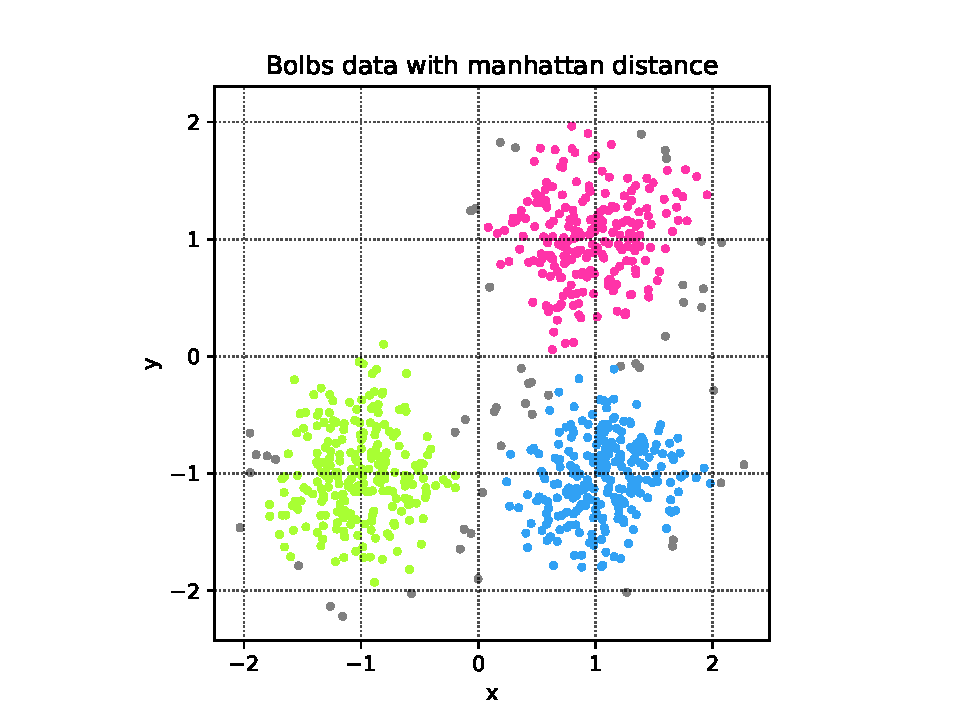
\includegraphics[width=\linewidth]{figures/4-bolb}  
		\caption{DBSCAN result in forth experiment}
		\label{fig:p2-1}
	\end{subfigure}
	\begin{subfigure}{0.33\textwidth}
		\centering
		% include image 2
		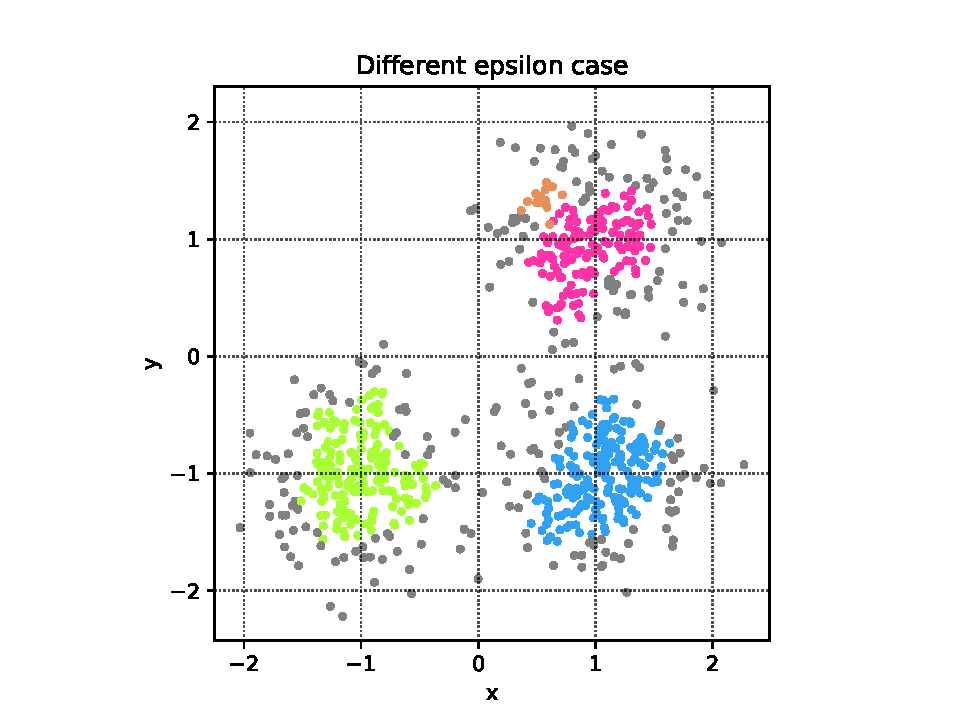
\includegraphics[width=\linewidth]{figures/5-epsilon}
		\caption{DBSCAN result in fifth experiment}
		\label{fig:p2-2}
	\end{subfigure}
	\begin{subfigure}{0.33\textwidth}
		\centering
		% include image 3
		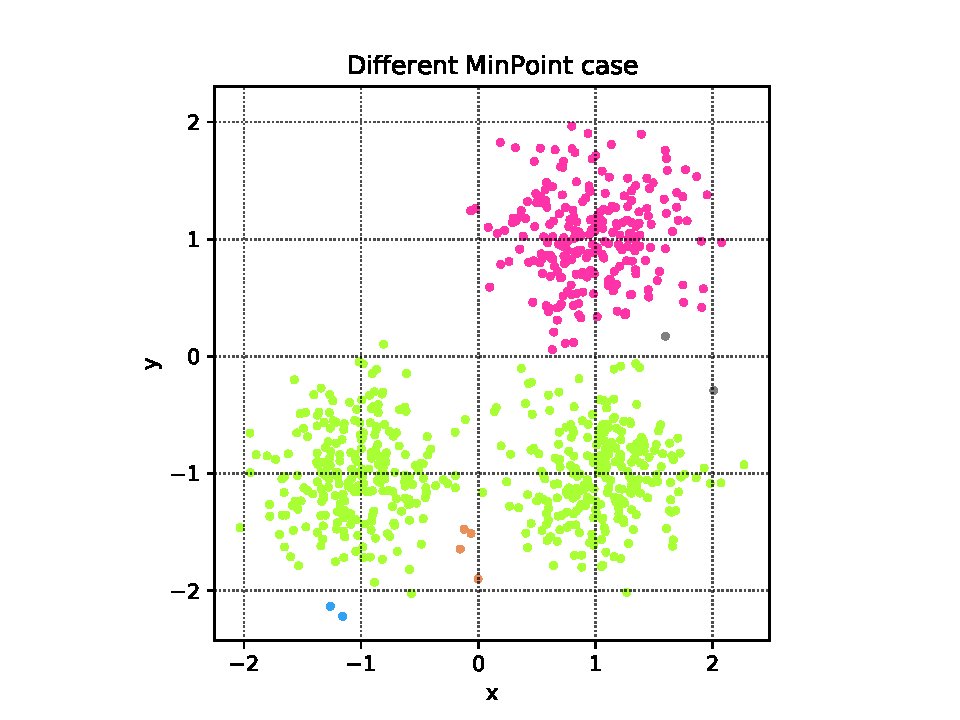
\includegraphics[width=\linewidth]{figures/6-MinPoint}
		\caption{DBSCAN result in sixth experiment}
		\label{fig:p2-3}
	\end{subfigure}	
	
	
	\begin{subfigure}{0.33\textwidth}
		\centering
		% include image 4
		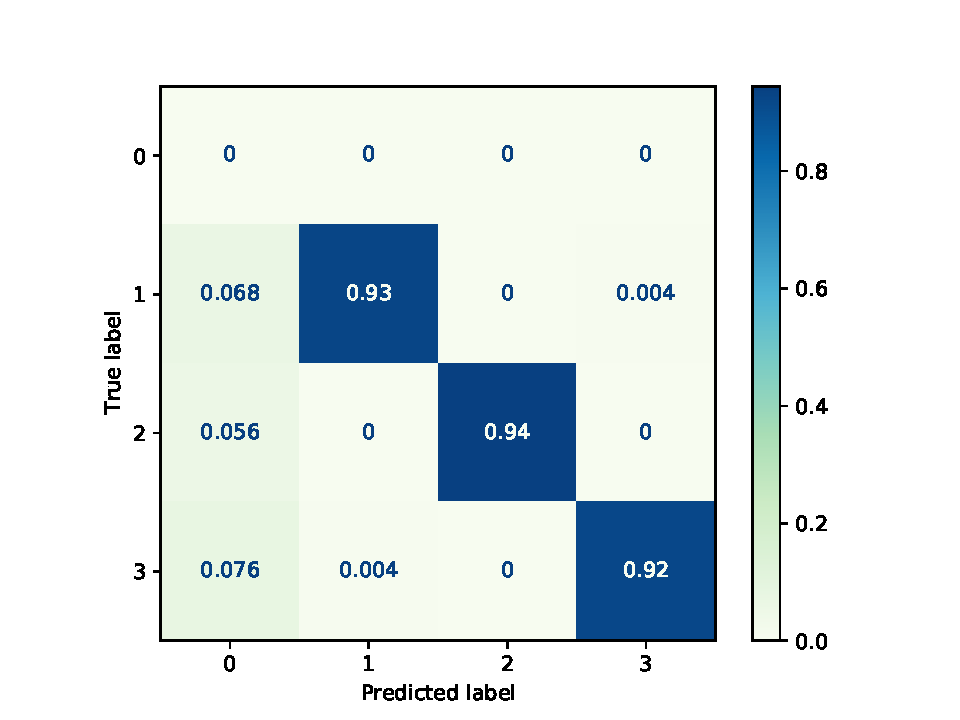
\includegraphics[width=\linewidth]{figures/4-cm_bolb}
		\caption{Confusion matrix of manhattan distance}
		\label{fig:p2-4}
	\end{subfigure}
	\begin{subfigure}{0.33\textwidth}
		\centering
		% include image 5
		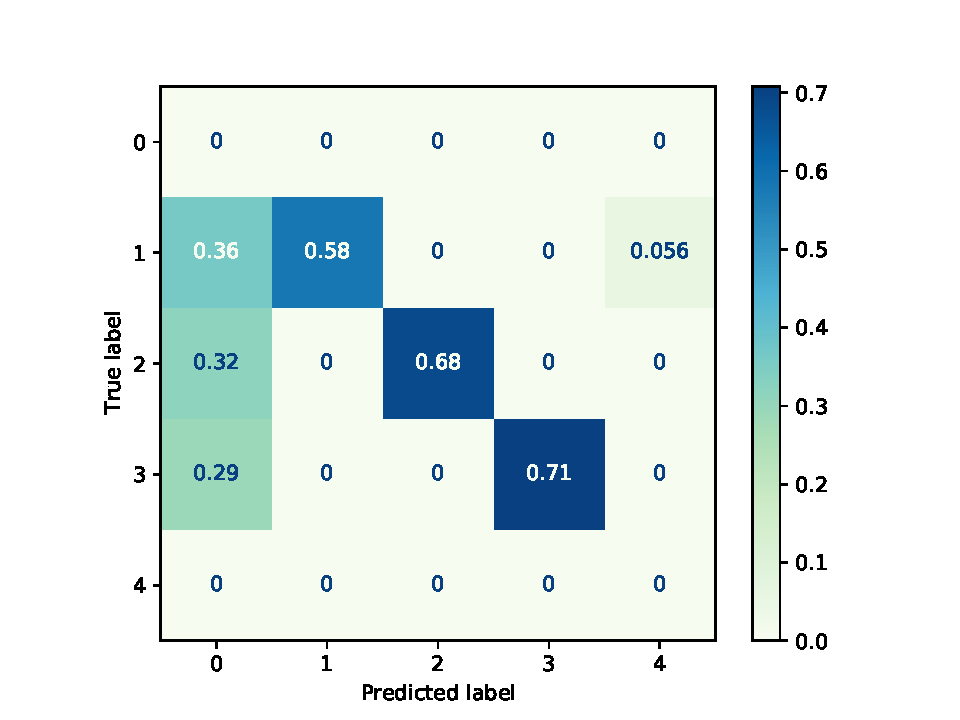
\includegraphics[width=\linewidth]{figures/5-cm-epsilon}  
		\caption{Confusion matrix of $\epsilon = 0.15$  }
		\label{fig:p2-5}
	\end{subfigure}
	\begin{subfigure}{0.33\textwidth}
		\centering
		% include image 6
		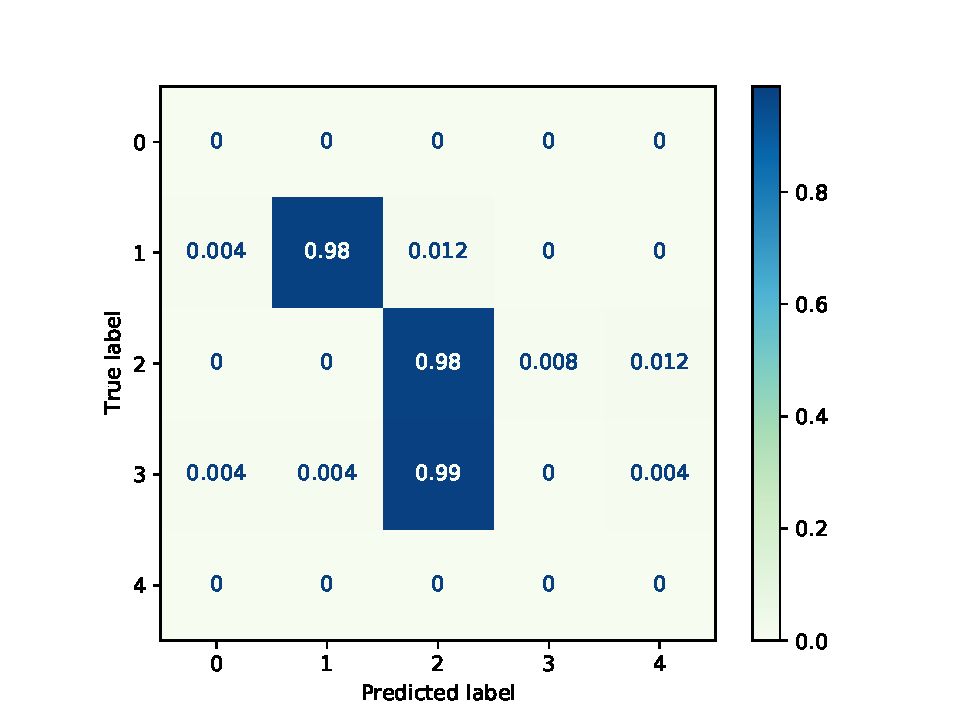
\includegraphics[width=\linewidth]{figures/6-cm-MinPoint}  
		\caption{Confusion matrix of MinPoint = 2 }
		\label{fig:p2-6}
	\end{subfigure}
	\caption{Result of second three experiment, here we change parameters of DBSCAN such as metric function, $\epsilon$ and MinPoint.}
	\label{fig:panel2}
\end{figure*}

in table \cref{tab:1,tab:2,tab:3,tab:4,tab:5,tab:6,tab:base} you can see the result of evaluating the clustering methods.
\begin{table}[]
	\centering
	\caption{Evaluation of base case accuracy was 0.97}
	\label{tab:base}
	\begin{tabular}{cccc}
		\textbf{Label} & \textbf{precision} & \textbf{recall} & \textbf{f1-score} \\
		\hline
		0 & 1.00 & 0.96 & 0.98 \\
		1 & 1.00 & 0.97 & 0.98 \\
		2 & 1.00 & 0.96 & 0.98
	\end{tabular}
\end{table}

\begin{table}[]
	\centering
	\caption{Evaluation of first case accuracy was 1.00}
	\label{tab:1}
	\begin{tabular}{cccc}
		\textbf{Label} & \textbf{precision} & \textbf{recall} & \textbf{f1-score} \\
		\hline
		0 & 1.00 & 1.00 & 1.00 
	\end{tabular}
\end{table}

\begin{table}[]
	\centering
	\caption{Evaluation of second case accuracy was 0.50}
	\label{tab:2}
	\begin{tabular}{cccc}
		\textbf{Label} & \textbf{precision} & \textbf{recall} & \textbf{f1-score} \\
		\hline
		0 & 0.50 & 1.00 & 0.67\\
		1 & 0.00 & 0.00 & 0.00
	\end{tabular}
\end{table}

\begin{table}[]
	\centering
	\caption{Evaluation of third case accuracy was 0.50}
	\label{tab:3}
	\begin{tabular}{cccc}
		\textbf{Label} & \textbf{precision} & \textbf{recall} & \textbf{f1-score} \\
		\hline
		0       &0.50 &     1.00  &    0.67 \\
		1       &0.00&      0.00   &   0.00 
	\end{tabular}
\end{table}

\begin{table}[]
	\centering
	\caption{Evaluation of forth case accuracy was 0.93}
	\label{tab:4}
	\begin{tabular}{cccc}
		\textbf{Label} & \textbf{precision} & \textbf{recall} & \textbf{f1-score} \\
		\hline
		  -1    &   0.00  &    0.00   &   0.00  \\       
			0    &   1.00  &    0.93   &   0.96  \\
			1    &   1.00  &    0.94   &   0.97  \\
			2    &  1.00   &    0.92   & 0.96    \\
	\end{tabular}
\end{table}

\begin{table}[]
	\centering
	\caption{Evaluation of fifth case accuracy was 0.66}
	\label{tab:5}
	\begin{tabular}{cccc}
		\textbf{Label} & \textbf{precision} & \textbf{recall} & \textbf{f1-score} \\
		\hline
          -1   &   0.00  &    0.00  &    0.00     \\
			0   &   1.00  &    0.98  &    0.99     \\
			1   &   0.49  &    0.98  &    0.66     \\
			2   &   0.00  &    0.00  &    0.00     \\
			3   &   0.00  &    0.00  &    0.00     \\
	\end{tabular}
\end{table}

\begin{table}[]
	\centering
	\caption{Evaluation of sixth case accuracy was 0.65}
	\label{tab:6}
	\begin{tabular}{cccc}
		\textbf{Label} & \textbf{precision} & \textbf{recall} & \textbf{f1-score} \\
		\hline
          -1    &   0.00   &   0.00    &  0.00     \\
			0    &   1.00   &   0.98    &  0.99     \\
			1    &   0.49   &   0.98    &  0.66     \\
			2    &   0.00   &   0.00    &  0.00     \\
			3    &   0.00   &   0.00    &  0.00     \\
	\end{tabular}
\end{table}


\begin{figure}[h]
	\centering
	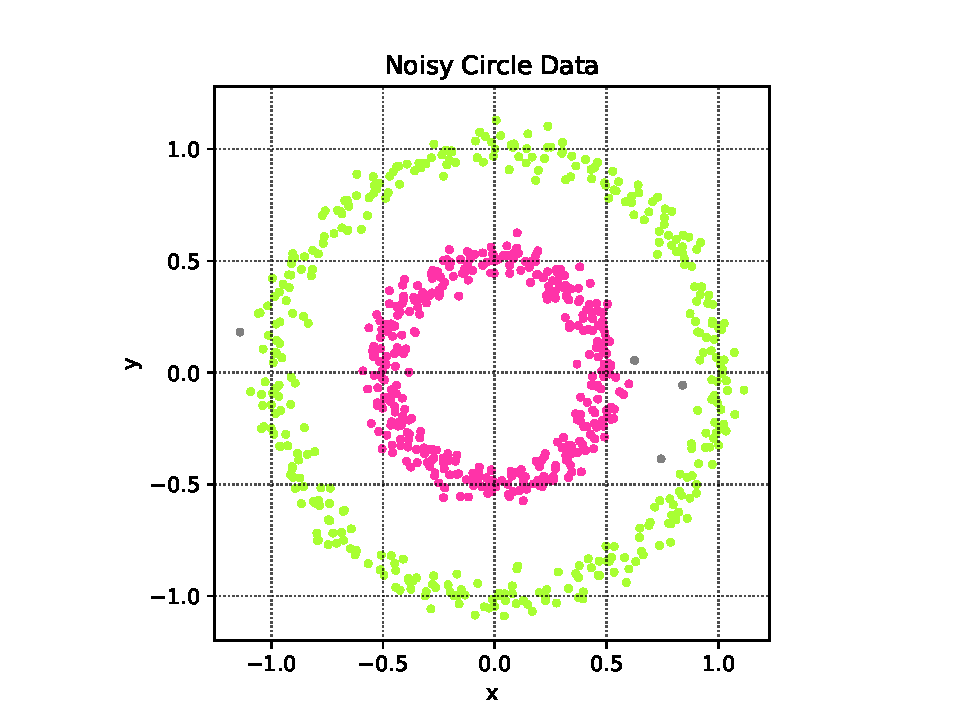
\includegraphics[width=1\linewidth]{figures/NoisyCircleTune}
	\caption{Noisy Cricle with $\epsilon = 0.1$ and MinPoint=3}
	\label{fig:noisycircletune}
\end{figure}

\begin{figure}[h]
	\centering
	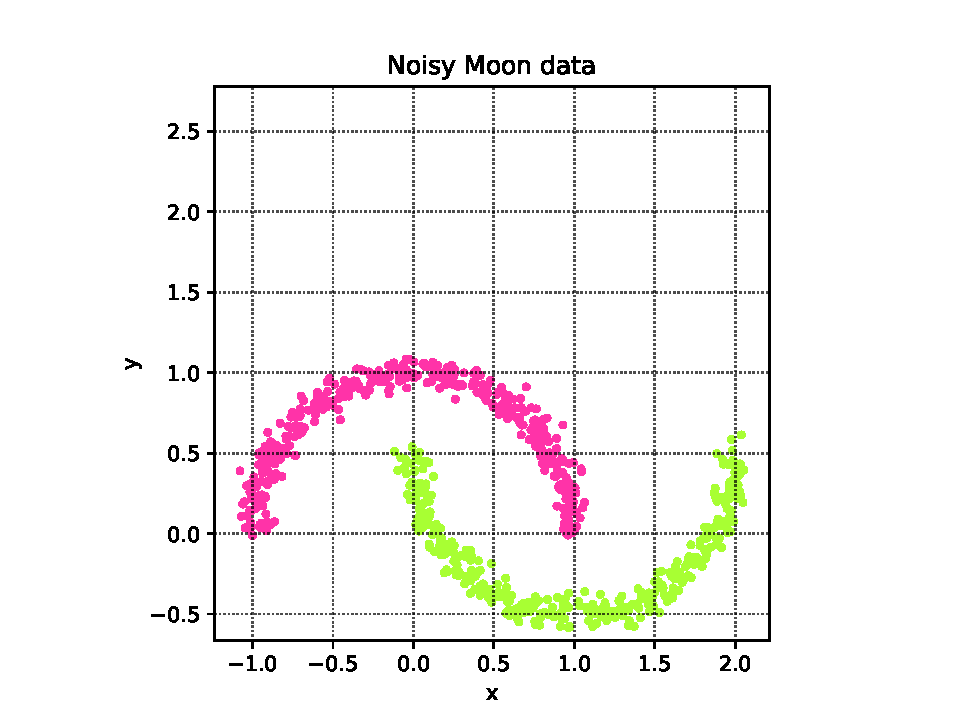
\includegraphics[width=1\linewidth]{figures/NoisyMoonTune}
	\caption{Noisy Moon with  $\epsilon = 0.3$ and MinPoint = 10}
	\label{fig:noisymoontune}
\end{figure}
